\section{Data Sources} 
\label{sec-data}

The type of data being compressed plays an important factor in how
well a compression algorithm will do.  Certain types of data will
favor one compression scheme over another compression scheme.  We
evaluate several compression schemes on three types of sensor data
collected from actual sensor network deployments.  

\subsection{Seismic Volcano Data}

We look at seismic data from a 19-day sensor network deployment at
Revenatador~\cite{volcano-osdi06}, an active volcano in Ecuador in
August of 2005.  Active volcanos produce many small earthquakes
throughout the day.  Monitoring and localizing these earthquakes allow
the volcanologists studying the volcano to make better predictions
about future eruptions from the volcano.  Telos motes were used to
collect seismic data from these earthquakes with a custom ADC sampling
board attached to the motes.  The seismic data was sampled at 100 Hz
and captured with 24 bits of resolution.  We looked at 229 earthquakes
over the 19 day period.  A sample of the data is shown in
Figure~\ref{fig:volcano-data}.

\begin{figure}[h]
  \centering
  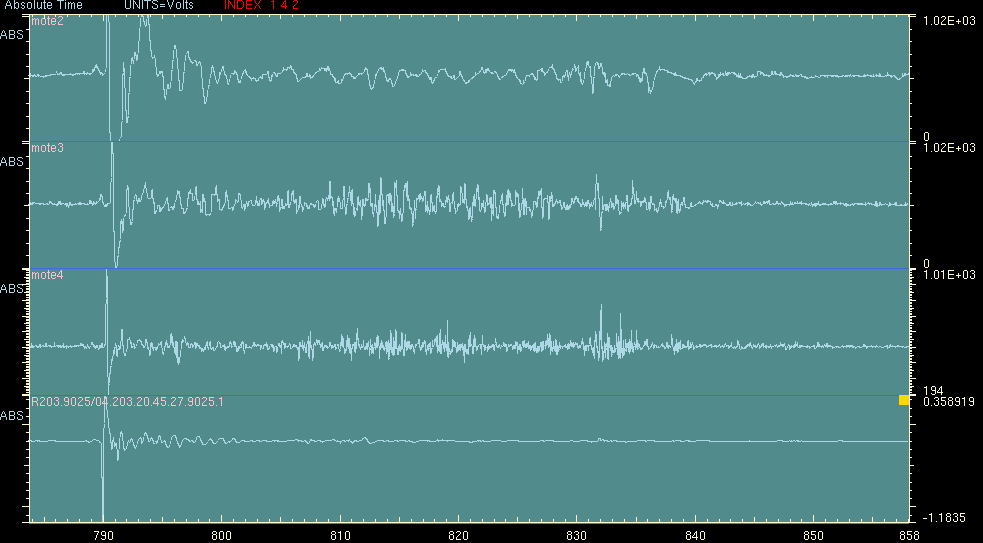
\includegraphics[width=0.75\textwidth]{figures/volcano-data.png} 
  \caption{Seismic data for four nodes at the start of an earthquake.}
  \label{fig:volcano-data}
\end{figure}

\subsection{Acoustic Data for Wildlife Habitat Tracking}

The second sensor data we look at is acoustic data from alarm calls
from yellow-bellied marmots at the Rocky Mountain Biological
Laboratory in Colorado~\cite{girod-marmots}.  These samples were
collected using the Acoustic ENSBox, a multi-node distributed
recording array.  Samples are collected from multiple microphones and
localization algorithms can pinpoint the position of the alarm call.
Data is sampled at a very high data rate of 24K samples per second.
Each sample is stored as a 16 bit signed sample.  A example of a
marmot alarm call is shown in Figure~\ref{fig:marmot-data}. 

\begin{figure}[h]
  \centering
  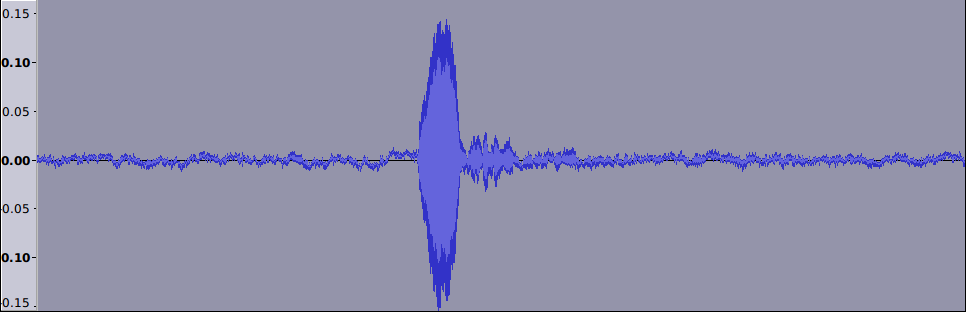
\includegraphics[width=0.75\textwidth]{figures/marmot-data.png} 
  \caption{An alarm call from a yellow-bellied marmot.}
  \label{fig:marmot-data}
\end{figure}

\subsection{Body Sensor Network Data}

Sensor networks have increasingly found themselves in medical
monitoring settings, such as monitoring patients with Parkinson's
Disease~\cite{parkinsons-embs07}, the most common neurodegenerative
disease, affecting about 3\% of the population over the age of 65.

Data was collected using the Intel Digital Health Group's Sensing
Health with Intelligence, Modularity, Mobilitiy, and Experimental
Reusability (SHIMMER) device.  The SHIMMER shares the same
micro-controller as the Telos motes (TI MSP430), and the same radio
(TI CC2420), but the SHIMMER platform has a built in three axis
accelerometer which when worn on the body, can capture movement of the
person.  There is also a daughter board which attaches to the SHIMMER
to get three axis of gyroscopic (angular motion) data from the patient
as well.  Both the accelerometer and gyroscope data is sampled from
the ADC on the MSP420 at 100 Hz and with 12 bits of resolution.
Sample data from a patient wearing one SHIMMER for one hour is shown
in Figure~\ref{fig:shimmer-data}.

\begin{figure}[h]
  \centering
  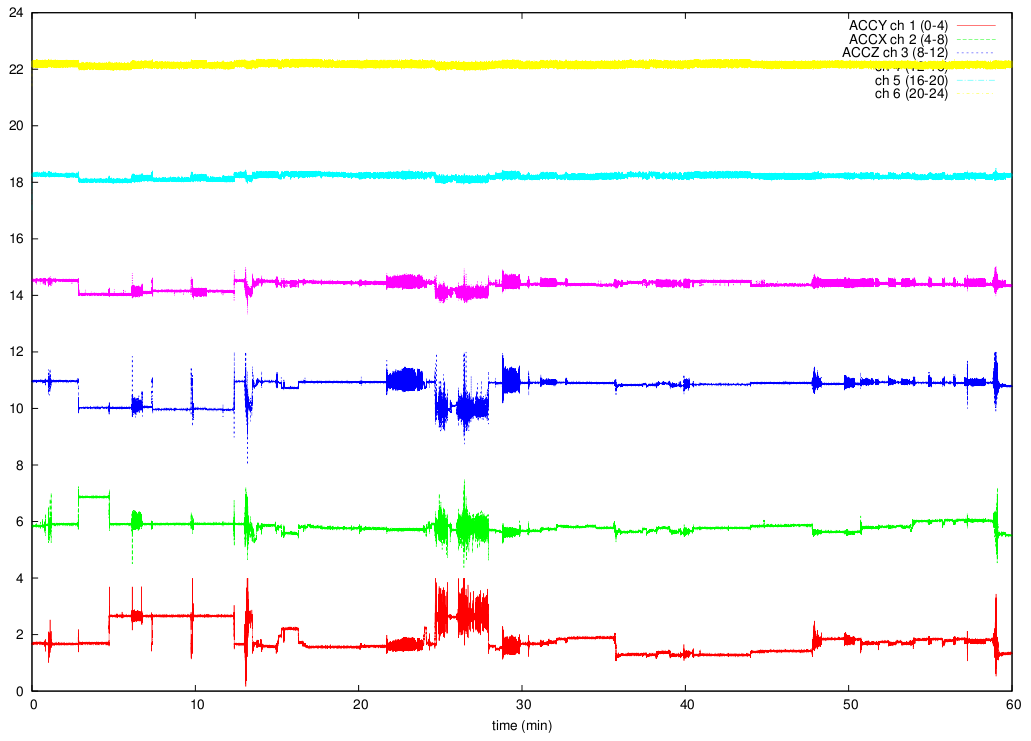
\includegraphics[width=0.75\textwidth]{figures/shimmer-data.png} 
  \caption{SHIMMER data for accelerometer and gryoscope.}
  \label{fig:marmot-data}
\end{figure}


